\PassOptionsToPackage{svgnames,dvipsnames,svgnames}{xcolor}

%% % From https://pldi19.sigplan.org/track/pldi-2019-papers#Call-for-Papers
%% \documentclass[sigplan,10pt,review,anonymous]{acmart}
%% \settopmatter{printfolios=true,printccs=false,printacmref=false}

%% For double-blind review submission, w/o CCS and ACM Reference (max submission space)
\documentclass[acmsmall,review,anonymous]{acmart}\settopmatter{printfolios=true,printccs=false,printacmref=false}
%% For double-blind review submission, w/ CCS and ACM Reference
%\documentclass[acmsmall,review,anonymous]{acmart}\settopmatter{printfolios=true}
%% For single-blind review submission, w/o CCS and ACM Reference (max submission space)
%\documentclass[acmsmall,review]{acmart}\settopmatter{printfolios=true,printccs=false,printacmref=false}
%% For single-blind review submission, w/ CCS and ACM Reference
%\documentclass[acmsmall,review]{acmart}\settopmatter{printfolios=true}
%% For final camera-ready submission, w/ required CCS and ACM Reference
%\documentclass[acmsmall]{acmart}\settopmatter{}


%% Conference information
%% Supplied to authors by publisher for camera-ready submission;
%% use defaults for review submission.
\acmConference[PL'18]{ACM SIGPLAN Conference on Programming Languages}{January 01--03, 2018}{New York, NY, USA}
\acmYear{2018}
\acmISBN{} % \acmISBN{978-x-xxxx-xxxx-x/YY/MM}
\acmDOI{} % \acmDOI{10.1145/nnnnnnn.nnnnnnn}
\startPage{1}

%% Copyright information
%% Supplied to authors (based on authors' rights management selection;
%% see authors.acm.org) by publisher for camera-ready submission;
%% use 'none' for review submission.
\setcopyright{none}
%\setcopyright{acmcopyright}
%\setcopyright{acmlicensed}
%\setcopyright{rightsretained}
%\copyrightyear{2018}           %% If different from \acmYear

%% Bibliography style
\bibliographystyle{ACM-Reference-Format}
%% Citation style
%\citestyle{acmauthoryear}  %% For author/year citations
%\citestyle{acmnumeric}     %% For numeric citations
%\setcitestyle{nosort}      %% With 'acmnumeric', to disable automatic
                            %% sorting of references within a single citation;
                            %% e.g., \cite{Smith99,Carpenter05,Baker12}
                            %% rendered as [14,5,2] rather than [2,5,14].
%\setcitesyle{nocompress}   %% With 'acmnumeric', to disable automatic
                            %% compression of sequential references within a
                            %% single citation;
                            %% e.g., \cite{Baker12,Baker14,Baker16}
                            %% rendered as [2,3,4] rather than [2-4].


%% Some recommended packages.
\usepackage{booktabs}   %% For formal tables:
                        %% http://ctan.org/pkg/booktabs
\usepackage{subcaption} %% For complex figures with subfigures/subcaptions
                        %% http://ctan.org/pkg/subcaption

%% Cyrus packages
\usepackage{microtype}
\usepackage{mdframed}
\usepackage{colortab}
\usepackage{mathpartir}
\usepackage{enumitem}
\usepackage{bbm}
\usepackage{stmaryrd}
\usepackage{mathtools}
\usepackage{leftidx}
\usepackage{todonotes}
\usepackage{xspace}
\usepackage{wrapfig}


\usepackage{listings}%
\lstloadlanguages{ML}
\lstset{tabsize=2, 
basicstyle=\footnotesize\ttfamily, 
% keywordstyle=\sffamily,
commentstyle=\itshape\ttfamily\color{gray}, 
stringstyle=\ttfamily\color{purple},
mathescape=false,escapechar=\#,
numbers=left, numberstyle=\scriptsize\color{gray}\ttfamily, language=ML, showspaces=false,showstringspaces=false,xleftmargin=15pt, 
morekeywords={string, float, int},
classoffset=0,belowskip=\smallskipamount, aboveskip=\smallskipamount,
moredelim=**[is][\color{red}]{SSTR}{ESTR}
}
\newcommand{\li}[1]{\lstinline[basicstyle=\ttfamily\fontsize{9pt}{1em}\selectfont]{#1}}
\newcommand{\lismall}[1]{\lstinline[basicstyle=\ttfamily\fontsize{9pt}{1em}\selectfont]{#1}}

%% Joshua Dunfield macros
\def\OPTIONConf{1}%
\usepackage{joshuadunfield}

%% Can remove this eventually
\usepackage{blindtext}

\usepackage{enumitem}

%%%%%%%%%%%%%%%%%%%%%%%%%%%%%%%%%%%%%%%%%%%%%%%%%%%%%%%%%%%%%%%%%%%%%%%%%%%%%
%% Matt says: Cyrus, this package `adjustbox` seems directly related
%% to the `clipbox` error; To get rid of the error, I moved it last
%% (after other usepackages) and I added the line just above it, which
%% permits it to redefine `clipbox` (apparently also defined in
%% `pstricks`, and due to latex's complete lack of namespace
%% management, these would otherwise names clash).
\let\clipbox\relax
\usepackage[export]{adjustbox}% http://ctan.org/pkg/adjustbox
%%%%%%%%%%%%%%%%%%%%%%%%%%%%%%%%%%%%%%%%%%%%%%%%%%%%%%%%%%%%%%%%%%%%%%%%%%%%%%%%%


%%%%%%%%%%%%%%%%%%%%%%%%%%%%%%%%%%%%%%%%%%%%%%%%%%%%%%%%%%%%%%%%%%%%%%%%%%%%%%%%%
%\usepackage{draftwatermark}
%\SetWatermarkText{DRAFT}
%\SetWatermarkScale{1}
%%%%%%%%%%%%%%%%%%%%%%%%%%%%%%%%%%%%%%%%%%%%%%%%%%%%%%%%%%%%%%%%%%%%%%%%%%%%%%%%%


% A macro for the name of the system being described by ``this paper''
\newcommand{\HazelnutLive}{\textsf{Hazelnut Live}\xspace}
\newcommand{\Hazelnut}{\textsf{Hazelnut}\xspace}
% The mockup, work-in-progress system.
\newcommand{\Hazel}{\textsf{Hazel}\xspace}

% \newtheorem{theorem}{Theorem}[chapter]
% \newtheorem{lemma}[theorem]{Lemma}
% \newtheorem{corollary}[theorem]{Corollary}
% \newtheorem{definition}[theorem]{Definition}
% \newtheorem{assumption}[theorem]{Assumption}
% \newtheorem{condition}[theorem]{Condition}

\newtheoremstyle{slplain}% name
  {.15\baselineskip\@plus.1\baselineskip\@minus.1\baselineskip}% Space above
  {.15\baselineskip\@plus.1\baselineskip\@minus.1\baselineskip}% Space below
  {\slshape}% Body font
  {\parindent}%Indent amount (empty = no indent, \parindent = para indent)
  {\bfseries}%  Thm head font
  {.}%       Punctuation after thm head
  { }%      Space after thm head: " " = normal interword space;
        %       \newline = linebreak
  {}%       Thm head spec
\theoremstyle{slplain}
\newtheorem{thm}{Theorem}  % Numbered with the equation counter
\numberwithin{thm}{section}
\newtheorem{defn}[thm]{Definition}
\newtheorem{lem}[thm]{Lemma}
\newtheorem{prop}[thm]{Proposition}
% \newtheorem{cor}[section]{Corollary}     
% \newtheorem{lem}[section]{Lemma}         
% \newtheorem{prop}[section]{Proposition}  

% \setlength{\abovedisplayskip}{0pt}
% \setlength{\belowdisplayskip}{0pt}
% \setlength{\abovedisplayshortskip}{0pt}
% \setlength{\belowdisplayshortskip}{0pt}



\makeatletter\if@ACM@journal\makeatother
%% Journal information (used by PACMPL format)
%% Supplied to authors by publisher for camera-ready submission
\acmJournal{PACMPL}
\acmVolume{1}
\acmNumber{1}
\acmArticle{1}
\acmYear{2018}
\acmMonth{3}
\acmDOI{10.1145/nnnnnnn.nnnnnnn}
\startPage{1}
\else\makeatother
%% Conference information (used by SIGPLAN proceedings format)
%% Supplied to authors by publisher for camera-ready submission
% \acmConference[]{ACM SIGPLAN Conference on Programming Languages}{January 01--03, 2017}{New York, NY, USA}

\acmYear{2018}
\acmISBN{978-x-xxxx-xxxx-x/YY/MM}
\acmDOI{10.1145/nnnnnnn.nnnnnnn}
\startPage{1}
\fi


%% Copyright information
%% Supplied to authors (based on authors' rights management selection;
%% see authors.acm.org) by publisher for camera-ready submission
\setcopyright{none}             %% For review submission
%\setcopyright{acmcopyright}
%\setcopyright{acmlicensed}
%\setcopyright{rightsretained}
%\copyrightyear{2017}           %% If different from \acmYear


\fancyfoot{} % suppresses the footer (also need \thispagestyle{empty} after \maketitle below)


%% Bibliography style
\bibliographystyle{ACM-Reference-Format}
%% Citation style
%% Note: author/year citations are required for papers published as an
%% issue of PACMPL.
\citestyle{acmauthoryear}   %% For author/year citations

% !TEX root = main.tex

\newcommand{\mynote}[3]{\textcolor{#3}{\textsf{{#2}}}}
\newcommand{\rkc}[1]{\mynote{rkc}{#1}{blue}}
\newcommand{\cy}[1]{\mynote{cy}{#1}{purple}}
\newcommand{\mah}[1]{\mynote{cy}{#1}{green}}
\newcommand{\matt}[1]{{\color{blue}{\textit{Matt:~#1}}}}

\newcommand{\cvert}{{\,{\vert}\,}}

%% https://tex.stackexchange.com/questions/9796/how-to-add-todo-notes
\newcommand{\rkcTodo}[1]{\todo[linecolor=blue,backgroundcolor=blue!25,bordercolor=blue]{#1}}

\newcommand{\mattTodo}[1]{\todo[linecolor=green,backgroundcolor=green!2,bordercolor=green]{\tiny\textit{#1}}}
\newcommand{\mattOmit}[1]{\colorbox{yellow}{(Matt omitted stuff here)}}

% \usepackage{amssymb}% http://ctan.org/pkg/amssymb
\usepackage{pifont}% http://ctan.org/pkg/pifont
\newcommand{\cmark}{\ding{51}}%
\newcommand{\xmark}{\ding{55}}%

\def\parahead#1{\paragraph{\textbf{#1.}}}
%% \def\paraheadNoDot#1{\paragraph{{\textbf{#1}}}}
\def\subparahead#1{\paragraph{\textit{#1.}}}
%% \def\paraheadindent#1{\paragraph{}\textit{#1.}}
%% \def\paraheadindentnodot#1{\paragraph{}\textit{#1}}

% \newcommand{\ie}{{\emph{i.e.}}}
% \newcommand{\eg}{{\emph{e.g.}}}
% \newcommand{\etc}{{\emph{etc.}}}
% \newcommand{\cf}{{\emph{cf.}}}
% \newcommand{\etal}{{\emph{et al.}}}

%% \newcommand{\hazel}{\ensuremath{\textsc{Hazel}}}
%% \newcommand{\sns}{\ensuremath{\textsc{Sketch-n-Sketch}}}
%% \newcommand{\deuce}{\ensuremath{\textsc{Deuce}}}
\newcommand{\Elm}{\ensuremath{\textsf{Elm}}}
\newcommand{\sns}
  %% {\ensuremath{\textrm{Sketch-n-Sketch}}}
  {\ensuremath{\textsf{Sketch-n-Sketch}}}
\newcommand{\deuce}
  %% {\ensuremath{\textrm{Deuce}}}
  {\ensuremath{\textsf{Deuce}}}

\newcommand{\sectionDescription}[1]{\section{#1}}
\newcommand{\subsectionDescription}[1]{\subsection{#1}}
\newcommand{\subsubsectionDescription}[1]{\subsubsection{#1}}
%% \newcommand{\subsectionDescription}[1]{\subsection*{#1}}
\newcommand{\suppMaterials}{the Supplementary Materials}

\newcommand{\defeq}{\overset{\textrm{def}}{=}}

\newcommand{\eap}{action suggestion panel\xspace}
\newcommand{\Eap}{Action suggestion panel\xspace}

\newcommand{\myfootnote}[1]{\footnote{ #1}}

\def\sectionautorefname{Section}
\def\subsectionautorefname{Section}
\def\subsubsectionautorefname{Section}

\newcommand{\code}[1]{\lstinline{#1}}

% Make italic?
%\newcommand{\Property}[1]{\emph{#1}}
\newcommand{\Property}[1]{\textrm{#1}}

% Calling out Cyrus's favorite verb, 'to be' ;)
\newcommand{\IS}{\colorbox{red}{is}\xspace}

\newcommand{\codeSize}
  %% {\footnotesize}
  {\small}

%\newcommand{\JoinTypes}[2]{\textsf{join}~~#1~~#2}
\newcommand{\JoinTypes}[2]{\textsf{join}(#1,#2)}

%%%%%%%%%%%%%%%%%%%%%%%%%%%%%%%%%%%%%%%%%%%%%%%%%%%%%%%%%%%%%%%%%%%%%%%%%%%%%%%%
%% Spacing

\newcommand{\sep}{\hspace{0.06in}}
\newcommand{\sepPremise}{\hspace{0.20in}}
\newcommand{\hsepRule}{\hspace{0.20in}}
\newcommand{\vsepRuleHeight}{0.08in}
\newcommand{\vsepRule}{\vspace{\vsepRuleHeight}}
\newcommand{\miniSepOne}{\hspace{0.01in}}
\newcommand{\miniSepTwo}{\hspace{0.02in}}
\newcommand{\miniSepThree}{\hspace{0.03in}}
\newcommand{\miniSepFour}{\hspace{0.04in}}
\newcommand{\miniSepFive}{\hspace{0.05in}}

%%%%%%%%%%%%%%%%%%%%%%%%%%%%%%%%%%%%%%%%%%%%%%%%%%%%%%%%%%%%%%%%%%%%%%%%%%%%%%%%

% \lstset{
% %mathescape=true,basicstyle=\fontsize{8}{9}\ttfamily,
% literate={=>}{$\Rightarrow$}2
%          {<=}{$\leq$}2
%          {->}{${\rightarrow}$}1
%          {\\\\=}{\color{red}{$\lambda$}}2
%          {\\\\}{$\lambda$}2
%          {**}{$\times$}2
%          {*.}{${\color{blue}{\texttt{*.}}}$}2
%          {+.}{${\color{blue}{\texttt{+.}}}$}2
%          {<}{${\color{green}{\lhd}}$}1
%          {>?}{${\color{green}{\rhd}}$?}2
%          {<<}{${\color{green}{\blacktriangleleft}}$}1
%          {>>?}{${\color{green}{\blacktriangleright}}$?}2
%          {\{}{${\color{blue}{\{}}$}1
%          {\}}{${\color{blue}{\}}}$}1
%          {[}{${\color{purple}{[}}$}1
%          {]}{${\color{purple}{]}}$}1
%          {(}{${\color{darkgray}{\texttt{(}}}$}1
%          {)}{${\color{darkgray}{\texttt{)}}}$}1
%          {]]}{${\color{gray}{\big(}}$}1
%          {]]}{${\color{gray}{\big)}}$}1
% }

% !TEX root = hazelnut-dynamics.tex

% \newcommand{\Label}[1]{\vspace{-20px}\label{#1}%
%   {\small\textcolor{cyan}{(\texttt{#1})}}\vspace{20px}%
% }

\newcommand{\cmttclo}[2]{\mathsf{clo}(#1, #2)}

% \newcommand{\CaptionLabel}[2]{
%   \caption{#1 {\small\textcolor{cyan}{(#2)}}}
%   \label{#2}}
\newcommand{\CaptionLabel}[2]{
  \caption{#1}
  \label{#2}}

% Violet hotdogs; highlight color helps distinguish them
\newcommand{\llparenthesiscolor}{\textcolor{violet}{\llparenthesis}}
\newcommand{\rrparenthesiscolor}{\textcolor{violet}{\rrparenthesis}}
% \newcommand{\llparenthesiscolor}{\textcolor{red}{\lfloor}}
% \newcommand{\rrparenthesiscolor}{\textcolor{red}{\rfloor}}

%% TODO if feeling really obsessive, use the following in place of x,u,c,b
\newcommand{\varVar}{x}
\newcommand{\varHole}{u}
\newcommand{\econst}{c}
\newcommand{\tbase}{b}

% HTyp and HExp
\newcommand{\isComplete}[1]{#1~\mathsf{complete}}

% HTyp
\newcommand{\tarr}[2]{#1 \rightarrow #2}
%\newcommand{\tsum}[2]{#1 + #2}
\newcommand{\tprod}[2]{#1 \times #2}
\newcommand{\tnum}{\texttt{num}}
\newcommand{\tb}{\texttt{b}}
\newcommand{\tehole}{\llparenthesiscolor\rrparenthesiscolor}
\newcommand{\tsum}[2]{{#1} + {#2}}

\newcommand{\tconsistent}[2]{#1 \sim #2}
\newcommand{\tinconsistent}[2]{#1 \nsim #2}

% HExp
\newcommand{\hlam}[2]{\lambda #1.#2}
\newcommand{\halam}[3]{\lambda #1{:}#2.#3}
\newcommand{\hap}[2]{#1(#2)}
\newcommand{\hapP}[2]{(#1)~(#2)} % Extra paren around function term
\newcommand{\hpair}[2]{(#1, #2)}
\newcommand{\hprj}[2]{\mathsf{prj}_{#1}(#2)}
\newcommand{\lblL}{\mathsf{L}}
\newcommand{\lblR}{\mathsf{R}}
\newcommand{\hnum}[1]{\underline{#1}}
%\newcommand{\hcase}[5]{\mathsf{case}\,#1\,\mathsf{of}\,#2\Rightarrow#3~\vert~#4\Rightarrow#5}
\newcommand{\hadd}[2]{#1 + #2}
\newcommand{\hehole}[1]{\llparenthesiscolor\rrparenthesiscolor^{#1}}
% \newcommand{\hhole}[1]{\setlength{\fboxsep}{0pt}\fcolorbox{red}{white}{\vphantom{)}$#1$}}
\newcommand{\hhole}[2]{\llparenthesiscolor#1\rrparenthesiscolor^{#2}}
% \newcommand{\hhole}[1]{
  % \setlength{\fboxsep}{0pt}
  % \colorbox{violet!10!white!100}{\ensuremath{\llparenthesiscolor#1\rrparenthesiscolor}}}
\newcommand{\hindet}[1]{\lceil#1\rceil}
%\newcommand{\hinj}[2]{\texttt{inj}_{#1}({#2})}
\newcommand{\hinL}[1]{\mathsf{inl}(#1)}
\newcommand{\hinR}[1]{\mathsf{inr}(#1)}
\newcommand{\hcase}[5]{\texttt{case}({#1},{#2}.{#3},{#4}.{#5})}

\newcommand{\hGamma}{\Gamma}
\newcommand{\EmptyhGamma}{\emptyset} % From hand-written notes, Canonical forms lemma; page 14
\newcommand{\EmptyDelta}{\cdot} % From hand-written notes, ES-Const rule, page 1
\newcommand{\domof}[1]{\text{dom}(#1)}
\newcommand{\hsyn}[3]{#1 \vdash #2 \Rightarrow #3}
\newcommand{\hana}[3]{#1 \vdash #2 \Leftarrow #3}

% ZTyp and ZExp
\newcommand{\zlsel}[1]{{\bowtie}{#1}}
\newcommand{\zrsel}[1]{{#1}{\bowtie}}

%\newcommand{\zwsel}[1]{\adjustbox{cframe=blue}{\ensuremath{{\textcolor{blue}{\triangleright}}{#1}{\textcolor{blue}{\triangleleft}}}}}
\newcommand{\zwsel}[1]{
  \setlength{\fboxsep}{0pt}
  \colorbox{green!10!white!100}{
    \ensuremath{{{\textcolor{Green}{{\hspace{-2px}\triangleright}}}}{#1}{\textcolor{Green}{\triangleleft{\vphantom{\tehole}}}}}}
}
%\newcommand{\zwsel}[1]{{\triangleright}{#1}{\triangleleft}}

\newcommand{\removeSel}[1]{#1^{\diamond}}

% ZTyp
\newcommand{\ztau}{\hat{\tau}}

% ZExp
\newcommand{\zexp}{\hat{e}}

% Direction
\newcommand{\dParent}{\mathtt{parent}}
\newcommand{\dChild}{\mathtt{firstChild}}
\newcommand{\dNext}{\mathtt{nextSib}}
\newcommand{\dPrev}{\mathtt{prevSib}}

% Action
\newcommand{\aMove}[1]{\mathtt{move}~#1}
	\newcommand{\zrightmost}[1]{\mathsf{rightmost}(#1)}
	\newcommand{\zleftmost}[1]{\mathsf{leftmost}(#1)}
\newcommand{\aSelect}[1]{\mathtt{sel}~#1}
\newcommand{\aDel}{\mathtt{del}}
\newcommand{\aReplace}[1]{\mathtt{replace}~#1}
\newcommand{\aConstruct}[1]{\mathtt{construct}~#1}
\newcommand{\aConstructx}[1]{#1}
\newcommand{\aFinish}{\mathtt{finish}}

\newcommand{\performAna}[5]{#1 \vdash #2 \xlongrightarrow{#4} #5 \Leftarrow #3}
\newcommand{\performAnaI}[5]{#1 \vdash #2 \xlongrightarrow{#4}\hspace{-3px}{}^{*}~ #5 \Leftarrow #3}
\newcommand{\performSyn}[6]{#1 \vdash #2 \Rightarrow #3 \xlongrightarrow{#4} #5 \Rightarrow #6}
\newcommand{\performSynI}[6]{#1 \vdash #2 \Rightarrow #3 \xlongrightarrow{#4}\hspace{-3px}{}^{*}~ #5 \Rightarrow #6}
\newcommand{\performTyp}[3]{#1 \xlongrightarrow{#2} #3}
\newcommand{\performTypI}[3]{#1 \xlongrightarrow{#2}\hspace{-3px}{}^{*}~#3}

\newcommand{\performMove}[3]{#1 \xlongrightarrow{#2} #3}
\newcommand{\performDel}[2]{#1 \xlongrightarrow{\aDel} #2}

% Form
\newcommand{\farr}{\mathtt{arrow}}
\newcommand{\fnum}{\mathtt{num}}
\newcommand{\fsum}{\mathtt{sum}}

\newcommand{\fasc}{\mathtt{asc}}
\newcommand{\fvar}[1]{\mathtt{var}~#1}
\newcommand{\flam}[1]{\mathtt{lam}~#1}
\newcommand{\fap}{\mathtt{ap}}
\newcommand{\farg}{\mathtt{arg}}
\newcommand{\fnumlit}[1]{\mathtt{lit}~#1}
\newcommand{\fplus}{\mathtt{plus}}
\newcommand{\fhole}{\mathtt{hole}}
\newcommand{\fnehole}{\mathtt{nehole}}

\newcommand{\finj}[1]{\mathtt{inj}~#1}
\newcommand{\fcase}[2]{\mathtt{case}~#1~#2}

% Talk about formal rules in example
\newcommand{\refrule}[1]{\textrm{Rule~(#1)}}

\newcommand{\herase}[1]{\left|#1\right|_\textsf{erase}}

\newcommand{\arrmatch}[2]{#1 \blacktriangleright_{\rightarrow} #2}
%% TODO maybe write underbracket
%% \newcommand{\groundmatch}[2]{\underline{#1} = #2}
\newcommand{\groundmatch}[2]{#1 \blacktriangleright_{\mathsf{ground}} #2}
\newcommand{\prodmatch}[2]{#1 \blacktriangleright_{\times} #2}
\newcommand{\summatch}[2]{#1 \blacktriangleright_{+} #2}


\newcommand{\TABperformAna}[5]{#1 \vdash & #2                & \xlongrightarrow{#4} & #5 & \Leftarrow #3}
\newcommand{\TABperformSyn}[6]{#1 \vdash & #2 \Rightarrow #3 & \xlongrightarrow{#4} & #5 \Rightarrow #6}
\newcommand{\TABperformTyp}[3]{& #1 & \xlongrightarrow{#2} & #3}

\newcommand{\TABperformMove}[3]{#1 & \xlongrightarrow{#2} & #3}
\newcommand{\TABperformDel}[2]{#1 \xlongrightarrow{\aDel} #2}

\newcommand{\sumhasmatched}[2]{#1 \mathrel{\textcolor{black}{\blacktriangleright_{+}}} #2}

%%%% DYNAMICS %%%%
%% TODO remove these macros
%% marks for eval
\newcommand{\unevaled}{\times}
\newcommand{\evaled}{\checkmark}
\newcommand{\markname}{m}

\newcommand{\mvar}[0]{u}
\newcommand{\subst}[0]{\sigma}
\newcommand{\substitute}[3]{[#1/#2]#3}
\newcommand{\fvof}[1]{\mathsf{FV}(#1)}
\newcommand{\dexp}[0]{d}
\newcommand{\dconst}[0]{c}
\newcommand{\dval}[0]{\ddot{v}}
%% TODO remove this macro
\newcommand{\dcast}[2]{\langle #1 \rangle ~ #2}
%% TODO make the following two look better
\newcommand{\dcasttwo}[3]{#1 \langle{#2}\Rightarrow{#3}\rangle}
\newcommand{\dcastthree}[4]
  {#1 \langle{#2}\Rightarrow{#3}\Rightarrow{#4}\rangle} %% sugared version
  %% {\dcasttwo{\dcasttwo{#1}{#2}{#3}}{#3}{#4}} %% unsugared version
\newcommand{\dcastfail}[3]{#1 \langle{#2}\Rightarrow{\tehole}\not\Rightarrow{#3}\rangle}
%% \newcommand{\dlam}[3]{\lambda #1:#2.#3}
\newcommand{\dlam}[3]{\halam{#1}{#2}{#3}}
\newcommand{\dap}[2]{#1(#2)}
\newcommand{\dapP}[2]{(#1)(#2)} % Extra paren around function term
\newcommand{\dnum}[1]{\underline{#1}}
%\newcommand{\dcase}[5]{\mathsf{case}\,#1\,\mathsf{of}\,#2\Rightarrow#3~\vert~#4\Rightarrow#5}
\newcommand{\dadd}[2]{#1 + #2}
%% TODO third arg should be empty
\newcommand{\dehole}[3]{\leftidx{^{#3}}{\llparenthesiscolor\rrparenthesiscolor}{^{#1}_{#2}}}
%% TODO fourth arg should be empty
\newcommand{\dhole}[4]{\leftidx{^{#4}}{\llparenthesiscolor#1\rrparenthesiscolor}{^{#2}_{#3}}}
\newcommand{\dindet}[1]{\lceil#1\rceil}
%\newcommand{\dinj}[2]{\texttt{inj}_{#1}({#2})}
\newcommand{\dinL}[2]{\mathsf{inl}_{#1}(#2)}
\newcommand{\dinR}[2]{\mathsf{inr}_{#1}(#2)}
\newcommand{\dcase}[5]{\texttt{case}({#1},{#2}.{#3},{#4}.{#5})}
\newcommand{\dpair}[2]{(#1,#2)}
\newcommand{\dprj}[2]{\mathsf{prj}_{#1}(#2)}

\newcommand{\expandAna}[6]{#1 \vdash #2 \Leftarrow #3 \leadsto #4 : #5 \dashv #6}
\newcommand{\expandSyn}[5]{#1 \vdash #2 \Rightarrow #3 \leadsto #4 \dashv #5}
\newcommand{\hasType}[4]{#1; #2 \vdash #3 : #4}
\newcommand{\isValue}[1]{#1~\mathsf{val}}
\newcommand{\isGround}[1]{#1~\mathsf{ground}}
\newcommand{\isBoxedValue}[1]{#1~\mathsf{boxedval}}
\newcommand{\isIndet}[1]{#1~\mathsf{indet}}
\newcommand{\isFinal}[1]{#1~\mathsf{final}}
\newcommand{\isErr}[2]{#1 \vdash #2~\mathsf{err}}
%% \newcommand{\stepsTo}[2]{#1 \mapsto_{\Delta} #2}
%% TODO first arg should be empty
%% \newcommand{\stepsToD}[3]{#1 \vdash #2 \mapsto #3}
\newcommand{\stepsToD}[3]{#2 \mapsto #3}
\newcommand{\multiStepsTo}[2]{#1 \mapsto^* #2}

%% TODO if feeling obsessive, replace direct uses of \Delta
\newcommand{\hDelta}{\Delta}
\newcommand{\Dunion}[2]{#1 \cup #2}
\newcommand{\idof}[1]{\mathsf{id}(#1)}
\newcommand{\Dbinding}[3]{#1 :: #3[#2]}
\newcommand{\instantiate}[3]{\llbracket#1 / #2\rrbracket #3}

% Contextual dynamics
\newcommand{\evalctx}{\mathcal{E}}
\newcommand{\evalhole}{\circ}
\newcommand{\isevalctx}[1]{#1~\mathsf{evalCtx}}
%% TODO first arg should be empty
%% \newcommand{\reducesE}[3]{#1 \vdash #2 \longrightarrow #3}
\newcommand{\reducesE}[3]{#2 \longrightarrow #3}
\newcommand{\selectEvalCtxR}[2]{#1\{#2\}}
\newcommand{\selectEvalCtx}[3]{#1=\selectEvalCtxR{#2}{#3}}
\newcommand{\maybePremise}[1]{{\textcolor{red}[}#1{\textcolor{red}]}}

\newcommand{\inhole}[2]{\mathsf{inhole}(#1; #2)}

\newcommand{\DoSubst}[3]{[#1/#2]{#3}}


\setlength{\abovecaptionskip}{4pt plus 3pt minus 2pt} % Chosen fairly arbitrarily
\setlength{\belowcaptionskip}{-4pt plus 3pt minus 2pt} % Chosen fairly arbitrarily


\begin{document}

%% Title information
%% \title{Live Hole Filling by Direct Manipulation}         %% [Short Title] is optional;
%% \title{Live and Direct Functional Programming \\with Palette Expressions}
\title
  [Programming with Direct Manipulation of Palette Expressions]
  {Programming with Direct Manipulation of\\Palette Expressions}
  %% [Programming by Direct Manipulation of Palettes]
  %% {Functional Programming by\\Direct Manipulation of Live Palette Expressions}

                                        %% when present, will be used in
                                        %% header instead of Full Title.
% \titlenote{with title note}             %% \titlenote is optional;
                                        %% can be repeated if necessary;
                                        %% contents suppressed with 'anonymous'
% \subtitle{Subtitle}                     %% \subtitle is optional
% \subtitlenote{with subtitle note}       %% \subtitlenote is optional;
                                        %% can be repeated if necessary;
                                        %% contents suppressed with 'anonymous'


%% Author information
%% Contents and number of authors suppressed with 'anonymous'.
%% Each author should be introduced by \author, followed by
%% \authornote (optional), \orcid (optional), \affiliation, and
%% \email.
%% An author may have multiple affiliations and/or emails; repeat the
%% appropriate command.
%% Many elements are not rendered, but should be provided for metadata
%% extraction tools.

%% Author with single affiliation.
\author{Cyrus Omar}
% \authornote{with author1 note}          %% \authornote is optional;
                                        %% can be repeated if necessary
% \orcid{nnnn-nnnn-nnnn-nnnn}             %% \orcid is optional
\affiliation{
  % \position{Position1}
  % \department{Department1}              %% \department is recommended
  \institution{University of Chicago}            %% \institution is required
  % \streetaddress{Street1 Address1}
  % \city{City1}
  % \state{State1}
  % \postcode{Post-Code1}
  % \country{Country1}
}
\email{comar@cs.uchicago.edu}          %% \email is recommended

\author{Ian Voysey}
% \authornote{with author1 note}          %% \authornote is optional;
                                        %% can be repeated if necessary
% \orcid{nnnn-nnnn-nnnn-nnnn}             %% \orcid is optional
\affiliation{
  % \position{Position1}
  % \department{Department1}              %% \department is recommended
  \institution{Carnegie Mellon University}            %% \institution is required
  % \streetaddress{Street1 Address1}
  % \city{City1}
  % \state{State1}
  % \postcode{Post-Code1}
  % \country{Country1}
}
\email{iev@cs.cmu.edu}          %% \email is recommended

\author{Ravi Chugh}
% \authornote{with author1 note}          %% \authornote is optional;
                                        %% can be repeated if necessary
% \orcid{nnnn-nnnn-nnnn-nnnn}             %% \orcid is optional
\affiliation{
  % \position{Position1}
  % \department{Department1}              %% \department is recommended
  \institution{University of Chicago}            %% \institution is required
  % \streetaddress{Street1 Address1}
  % \city{City1}
  % \state{State1}
  % \postcode{Post-Code1}
  % \country{Country1}
}
\email{rchugh@cs.uchicago.edu}          %% \email is recommended

\author{Matthew A. Hammer}
% \authornote{with author1 note}          %% \authornote is optional;
                                        %% can be repeated if necessary
% \orcid{nnnn-nnnn-nnnn-nnnn}             %% \orcid is optional
\affiliation{
  % \position{Position1}
  % \department{Department1}              %% \department is recommended
  \institution{University of Colorado Boulder}            %% \institution is required
  % \streetaddress{Street1 Address1}
  % \city{City1}
  % \state{State1}
  % \postcode{Post-Code1}
  % \country{Country1}
}
\email{matthew.hammer@colorado.edu}          %% \email is recommended


% %% Author with two affiliations and emails.
% \author{First2 Last2}
% \authornote{with author2 note}          %% \authornote is optional;
%                                         %% can be repeated if necessary
% \orcid{nnnn-nnnn-nnnn-nnnn}             %% \orcid is optional
% \affiliation{
%   \position{Position2a}
%   \department{Department2a}             %% \department is recommended
%   \institution{Institution2a}           %% \institution is required
%   \streetaddress{Street2a Address2a}
%   \city{City2a}
%   \state{State2a}
%   \postcode{Post-Code2a}
%   \country{Country2a}
% }
% \email{first2.last2@inst2a.com}         %% \email is recommended
% \affiliation{
%   \position{Position2b}
%   \department{Department2b}             %% \department is recommended
%   \institution{Institution2b}           %% \institution is required
%   \streetaddress{Street3b Address2b}
%   \city{City2b}
%   \state{State2b}
%   \postcode{Post-Code2b}
%   \country{Country2b}
% }
% \email{first2.last2@inst2b.org}         %% \email is recommended


%% Paper note
%% The \thanks command may be used to create a "paper note" ---
%% similar to a title note or an author note, but not explicitly
%% associated with a particular element.  It will appear immediately
%% above the permission/copyright statement.
% \thanks{with paper note}                %% \thanks is optional
                                        %% can be repeated if necesary
                                        %% contents suppressed with 'anonymous'


%% Abstract
%% Note: \begin{abstract}...\end{abstract} environment must come
%% before \maketitle command
% !TEX root = palettes-paper.tex

\begin{abstract}

Palettes... \cite{popl-paper}

\end{abstract}



%% 2012 ACM Computing Classification System (CSS) concepts
%% Generate at 'http://dl.acm.org/ccs/ccs.cfm'.
% \begin{CCSXML}
% <ccs2012>
% <concept>
% <concept_id>10011007.10011006.10011008</concept_id>
% <concept_desc>Software and its engineering~General programming languages</concept_desc>
% <concept_significance>500</concept_significance>
% </concept>
% <concept>
% <concept_id>10003456.10003457.10003521.10003525</concept_id>
% <concept_desc>Social and professional topics~History of programming languages</concept_desc>
% <concept_significance>300</concept_significance>
% </concept>
% </ccs2012>
% \end{CCSXML}

% \ccsdesc[500]{Software and its engineering~General programming languages}
% \ccsdesc[300]{Social and professional topics~History of programming languages}
%% End of generated code


%% Keywords
%% comma separated list
% \keywords{keyword1, keyword2, keyword3}  %% \keywords is optional
\keywords{Live Programming, Palettes, Hazel, Code Editors}


%% \maketitle
%% Note: \maketitle command must come after title commands, author
%% commands, abstract environment, Computing Classification System
%% environment and commands, and keywords command.
\maketitle
\thispagestyle{empty} % suppresses the footer

\setcounter{section}{-1}
\section{TODO List}

\begin{itemize}

\item[\cmark] palette macros
\item action semantics
\item \Hazel{} in \Hazel{} (sums, productions, recursive types)
\item palette functions
\item live palettes
\item synthetic (or fancy record-type-level-computation) (or not-fancy untyped) palettes
\item parameterized palettes
\item palette-specific actions
\item option to render palette macro expansion as expression or value
\item \Hazel{} UI: ``formula bar'' for expressions
\item \sns{} implementation
\item examples!

\end{itemize}

\clearpage
\section{Introduction}\label{sec:intro}
Text-based program editors are flexible and expressive user interfaces
so it is little wonder that they remain dominant decades after the teletype.
However, textual user interfaces are not the best tool for every computational job.
% In particular, there are countless 
% data types for which a non-textual
% user interface may situationally be more appropriate.

As a simple example, consider a record type
classifying RGBA-encoded colors. 
It is possible to select a particular color by entering
an expression of this type in a text editor, e.g. \li{\{ r: 255, g: 178, b: 45, a: 100 \}}. 
The problem with this textual user interface for color selection is that 
it offers no live feedback about which color has been selected 
and limited editing affordances for tweaking the selected color.
Analagous critiques apply to strictly textual user interfaces for 
countless other data structures,
such as vector graphics,
animation parameters,
musical sequences,
audio filters,
board game states, 
GUI widgets and layouts,
tabular data, 
plots,
geospatial data, 
neural network diagrams, 
biological neuron models, 
mathematical diagrams, 
and so on.

% It is difficult for the programmer, or anyone subsequently reading or modifying the code, to know which color is represented
% and to interactively tweak that color.

Practitioners in domains where manipulating data of types like these is 
a central activity 
have largely eschewed general-purpose programming environments 
in favor of more specialized graphical end-user applications, like %
image and video editors, music composition software, level design tools, 
and bespoke GUIs written by students or lab technicians, 
in large part because these applications 
take seriously the need for domain-specific forms of live feedback, 
graphical data representations, and 
direct manipulation affordances, 
e.g. color palettes, visual timelines, interactive plots, and maps.

The tragedy is that these applications have 
limited support for abstraction and composition.
It is difficult, for example, to bind a
color to a variable for use in multiple locations in an
otherwise directly constructed game map,
or to define a function that computes portions of an 
otherwise directly constructed vector graphic,
or to transform a directly constructed musical sequence 
by passing it through a series of symbolically defined functions.
Moreover, it is difficult to add new affordances or to compose
affordances in ways that the application developer did not anticipate.
Users cannot easily make even simple changes like replacing a numeric text box in a dialog with a slider,
much less more ambitious changes like installing an alternative visual interface for expressing geospatial data queries 
into a database frontend.

% Better support for manipulating data of types like these would be particularly helpful for users engaging in
% live and exploratory programming in domains like web design, media production,
% and data analysis. Indeed, 

This paper aims to resolve this tension between
programmatic and direct manipulation user interfaces by designing 
a programming environment that
is able to surface GUIs when working with types for which
they are useful, while retaining full support for symbolic program manipulation
and the abstraction and composition mechanisms
available in modern general-purpose programming languages.

\subsection{Background}\label{sec:background}
\definecolor{mygray}{rgb}{0.93, 0.93, 0.93}
\definecolor{shadecolor}{named}{mygray}

\begin{figure*}
  \begin{minipage}[t]{0.37\textwidth}
    \begin{subfigure}[t]{\linewidth}
    \begin{snugshade}
      \vspace*{-2mm}
      \caption{\textbf{Prior Work:} Graphite \cite{Graphite}}
       \label{fig:graphite}
      \vspace*{1mm}
     \end{snugshade}
      \vspace*{-1mm}
      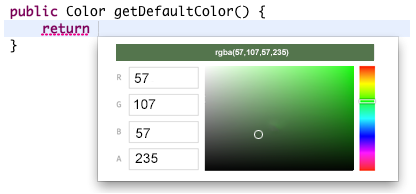
\includegraphics[width=\linewidth]{graphite-color-palette-green.png}
      \vspace*{-5mm}
    \end{subfigure}
    \hspace{8mm}
    \begin{subfigure}[t]{\linewidth}
     \begin{snugshade}
      \vspace*{-2mm}
      \caption{\textbf{This Paper:} Livelits are live and compositional}
    \label{fig:color}
      \vspace*{1mm}
     \end{snugshade}
      \vspace*{-1mm}
      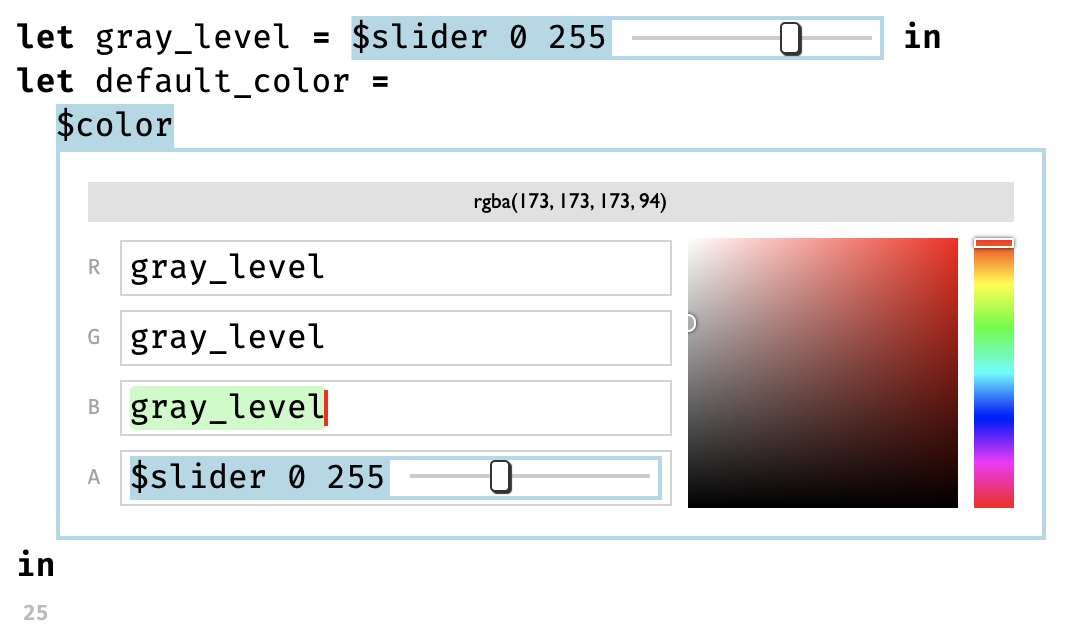
\includegraphics[width=\linewidth]{slider-color-livelits.png}
    \end{subfigure}
  \end{minipage}
  \hspace{10.5mm}
  \begin{subfigure}[t]{0.50\textwidth}
  \begin{snugshade}
   \vspace*{-2mm}
    \caption{\textbf{Case Study}: Grading with Livelits}
    \label{fig:grading}
    \vspace*{1mm}
     \end{snugshade}
    \vspace*{-1mm}
    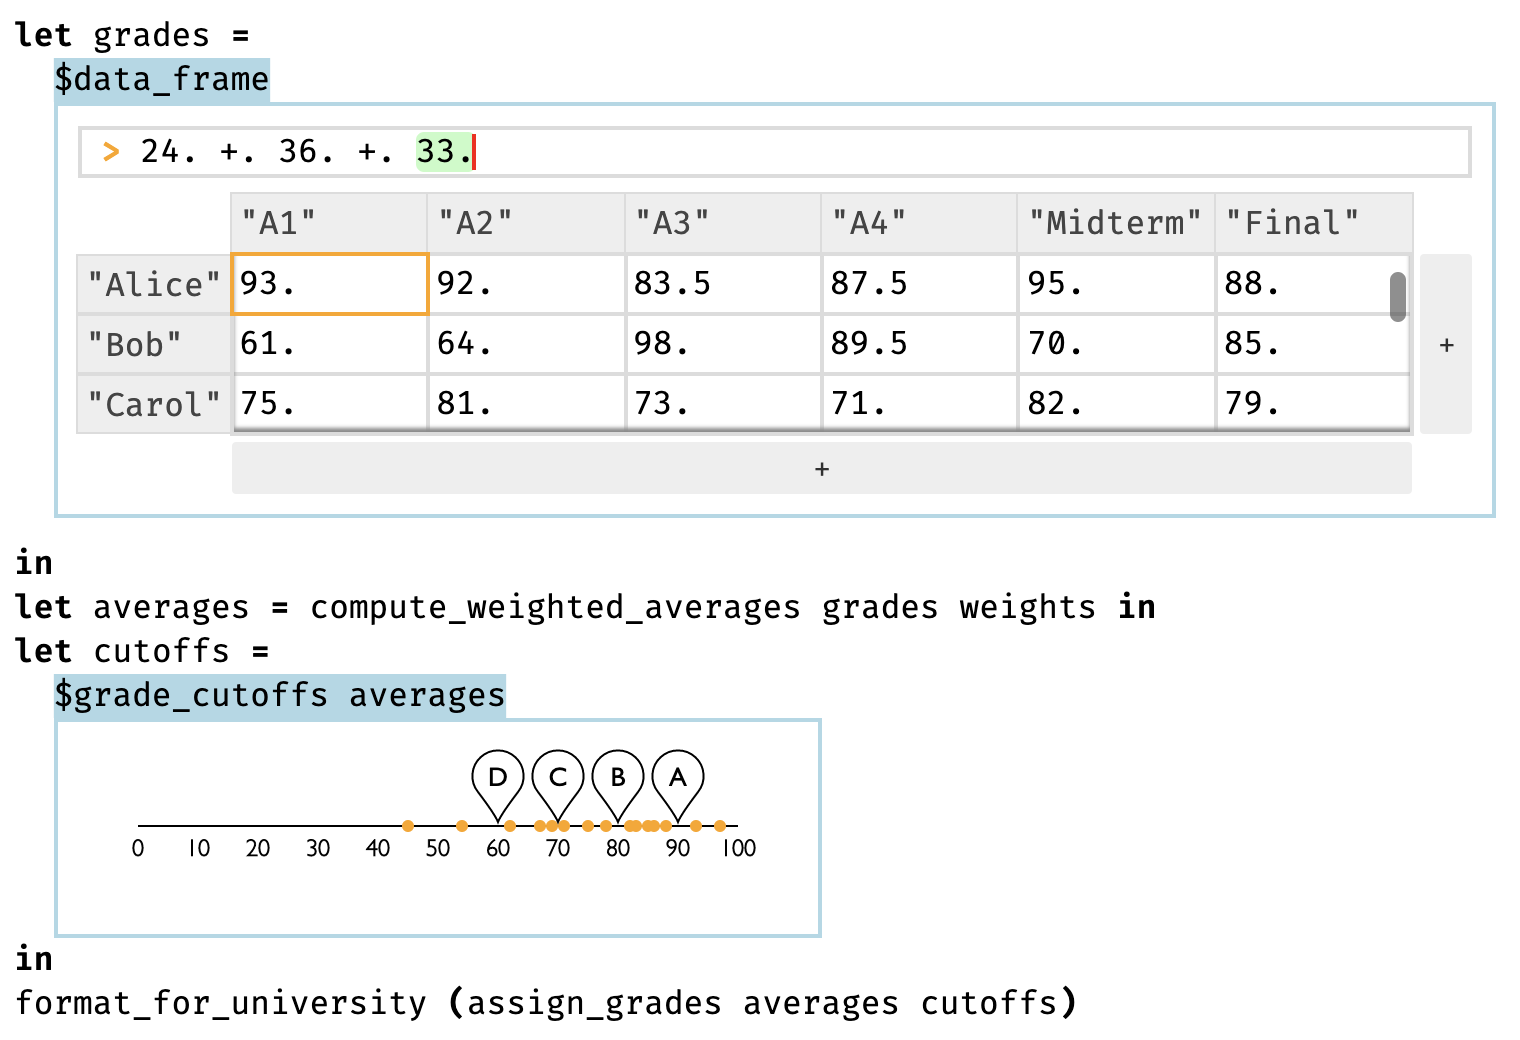
\includegraphics[width=\linewidth]{grade-cutoff-livelit.png}
  \end{subfigure}
  \vspace{-4mm}
   \caption{Introductory Examples}
%   \vspace*{-2mm}
\end{figure*}

Of course, we are not the first to integrate direct manipulation interfaces
into symbolic programming environments.
% Prior work on projectional editing
% and active code completion, detailed in Sec. \ref{sec:related-work},
% has also considered the problem of entering expressions
% of certain types, like \li{Color},
% using specialized GUIs integrated into a program editor.
% We detail prior work in Sec.~\ref{sec:related-work}, but 
The prior work most relevant to this paper is the {Graphite} system for Eclipse for Java,
demonstrated in Fig.~\ref{fig:graphite} \cite{Graphite}.
Graphite allows a library provider to associate a GUI, called a \emph{palette}, with a type 
(via a Java class annotation).
Wherever an expression of this type is needed,
i.e. wherever there is a \emph{hole} of that type in the program
(as determined by Eclipse's online parser and typechecker),
the environment offers the client the option, via the code completion menu,
to interact with the palette.
Once the interaction is finished, the palette generates a
Java expression to fill the hole.
Figure~\ref{fig:graphite}, adapted from this prior work, demonstrates a color palette invoked using Graphite.
When the user presses the \li{Enter} key, the Java expression \li{new Color(173, 173, 173, 85)} is inserted at the cursor and the palette disappears.
Several related systems, such as the  
\textbf{mage} system for the Jupyter notebook environment \cite{DBLP:conf/uist/KeryRHMWP20}
behave fundamentally similarly.
Projectional editing, the visual macro system in Racket \cite{interactive-visual-syntax}, and a number of other designs
also confront this general problem of integrating GUIs and code.

\citet{Graphite} evaluated Graphite by surveying 473 developers 
and \citet{DBLP:conf/uist/KeryRHMWP20} evaluated \textbf{mage} by interviewing 9 developers.
Both studies found that
participants viewed the proposed mechanism favorably and 
would use a suitable GUI some or all of the time.
% \footnote{When presented with a color palette,
% many participants remarked that they rarely entered colors directly into Java code,
% but rather into stylesheets.
% Other palettes, e.g. a palette
% that supported regular expression construction, were viewed as more
% suitable for Java code.
% The mechanisms being considered are suitable both for general-purpose languages
% and typed domain-specific languages like typed stylesheets, which can often be embedded into modern
% general-purpose languages.}
This and other prior work also collectively showcase a wide variety of use cases \cite{Graphite,DBLP:conf/uist/KeryRHMWP20,interactive-visual-syntax}, 
and the Graphite survey solicited dozens of additional use cases from participants,
which the authors systematically taxonomize \cite{Graphite}. 
We take these extensive empirical findings   
as evidence for, and a showcase of, 
the value of this class of mechanisms for integrating GUIs into code.
\vspace{-1mm}
\subsection{Contributions}
\label{sec:contributions}
We turn our attention in this paper to several fundamental technical
deficiencies that limit GUI providers and clients using these prior systems.
To address these, 
we introduce a system of \emph{live literals}, or \emph{livelits}, 
demonstrated in Fig.~\ref{fig:color}. 
Livelits are unique in achieving all of the following properties.
(We describe which subset of these properties 
are achieved by prior systems,
including those just mentioned, 
in Sec.~\ref{sec:related-work}.)

\newcommand{\llproperty}[1]{\vspace{5px}\noindent\textbf{#1}.}

\llproperty{Decentralized Extensibility}
    Providers define livelits in libraries, and 
    clients invoke livelits by name. Livelit names, e.g. \li{\$color},  are prefixed by \li{\$},    
    to distinguish them from variables.
    % We call this \emph{decentralized extensibility}.
    % Both mage and Racket's visual syntax system are similarly extensible, 
    % but 
    % In Graphite, palettes are associated with class definitions, 
    % so there is a tighter association between 
    % Other systems, discussed in Sec.~\ref{sec:related-work}, 
    % are either non-extensible, or cannot be extended by library providers 
    % (only by, for example, separately installed editor extensions, or by 
    % regenerating the editor using a language workbench.)
 
\llproperty{Persistence}
  % In Graphite and \textbf{mage}, GUIs are {ephemeral},
  % i.e. they disappear after the initial interaction,
  % leaving behind only the generated textual code.
  % Only the programmer that initially enters the expression
  % benefits from the feedback and affordances that the GUI provides.
  % %
  % \footnote{Graphite does include an \emph{ad hoc} mechanism that
  % allows palettes to parse the code that is selected in the editor
  % when the palette loads, but this requires that each palette implement
  % a parser for the subset of Java used in the code that it generates,
  % and therefore this mechanism is quite brittle. It is also difficult
  % to persist GUI state that is not included in the generated code.}
  Livelits are persistent elements of the syntax tree. They operate as  
  graphical literals, rather than as the ephemeral code generation GUIs of Graphite and \textbf{mage}. 
  We define a pure model-view-update-expand architecture
  (a variation on Elm's model-view-update architecture \cite{ElmArchitecture}) 
  where only the model needs to be persisted.
  The dynamic meaning of a livelit is determined by macro expansion.
  % We chose the word ``literal'' rather than ``palette'' because,  persistence, livelits
  % operate as graphical literals.

\llproperty{Hygienic Composition}
% Prior systems have limited or no support for {entering sub-expressions within the GUI}, 
% so they are useful mainly for generating expressions composed of constants,
% e.g. color constants in Fig.~\ref{fig:color}(a).
%
  Livelits support sub-expressions directly in the GUI, which we call \emph{splices} (after
   \citet{TLMs}).
  Fig.~\ref{fig:color} demonstrates splicing: the RGBA components  
  are splice editors, so the client can define a variable, \li{baseline},
  to relate the color components 
  and use a slider livelit inline to specify the alpha component.
  % Similarly, Fig.~\ref{fig:grading}(b)\todo{subfigure labels}{} demonstrates a 
  %  data table livelit where each entry is a splice.
  
  Crucially, composition is strictly 
  governed by a hygiene discipline that ensures
  (1) \textbf{capture avoidance}, i.e. that variables that the client uses in splices 
  will not capture expansion-internal bindings; and 
  (2) \textbf{context independence}, i.e. that the livelit 
  can be invoked in any program context.%without pre-condition or conflict.

\llproperty{Parameterization} Livelits can form parameterized families.
  For example, \li{\$slider} in Fig.~\ref{fig:color} is parameterized by the slider's bounds.
  Parameters operate like splices, differing in that they can be partially applied in
  livelit abbreviations. For example, Fig.~\ref{fig:color}
  partially applies \li{\$slider} to \li{0} and \li{100} to define a \li{\$percent} slider.
  % \begin{lstlisting}[numbers=none]
  % let $percentage = $slider 0 100 in ...
  % \end{lstlisting}
  % Parameterization also underlies the hygiene mechanism, as we will discuss in Sec.~\ref{sec:livelit-definitions}.

\llproperty{Typing} Each livelit specifies the type of expansions it generates, 
and parameters and splices also specify types, 
so livelits are compatible with type-driven methodologies and tools.
Together with the hygiene discipline, this allow clients to reason abstractly about expansions, i.e.  
without inspecting the expansions or livelit implementations directly.

\llproperty{Liveness} Uniquely, livelits can evaluate splices 
  throughout the editing process 
  (i.e. in a \emph{live} manner \cite{DBLP:conf/icse/Tanimoto13}) 
  to provide feedback related to run-time behavior.
  For example, in Fig.~\ref{fig:color}, 
  displaying the selected color requires evaluating the RGBA
  component splices to numeric values.
  Evaluation occurs in a run-time environment (i.e. closure) determined by
  leaving the hole being filled by the livelit temporarily unfilled and then evaluating
  using a two-phased variant of the semantics for 
  live programming with typed holes developed by \citet{HazelnutLive}.
  We support live evaluation even for livelits 
  that appear inside a function. Multiple function calls lead 
  to multiple closures that the client 
   can select between.

\paragraph{Outline.} We begin in Sec.~\ref{sec:case-studies} by introducing
livelits from the perspective of client programmers. 
Our examples are organized into case studies 
and are chosen to demonstrate the novel contributions of this paper.
In Sec.~\ref{sec:livelit-definitions}, 
we consider the livelit provider's perspective by introducing livelit
definitions with a detailed example.
In Sec.~\ref{sec:livelit-calculus}, we define the \emph{typed livelit calculus}. 
We have mechanically specified the central mechanism, livelit expansion, and proven the associated metatheorems in Agda.
This calculus 
serves to capture the essential nature of livelits 
independent of the particularities of syntax, GUI frameworks, 
and other orthogonal design details,
because we believe livelits can be integrated into a wide variety of programming systems. 
In Sec.~\ref{sec:implementation}, we provide a more detailed account of our two implementations of livelits.
Our primary implementation, used in the screenshots in the paper,
is integrated into Hazel, a live programming environment designed 
around hole-driven development. 
We have also prototyped livelits within a standard text editor. 
Additionally, we discuss factors that must be considered when integrating livelits into languages with side effects.
In Sec.~\ref{sec:related-work}, we compare livelits to related work using the design properties outlined above 
as a rubric.
Finally, we conclude in Sec.~\ref{sec:discussion} after a discussion of present limitations and future work.

\clearpage
\section{Overview Examples: Using Palettes}
\label{sec:overview}

\begin{figure*}


\includegraphics[scale=0.50]{images/MrSmileyFace.png}

\caption{Example Palettes in Hazel.}
\end{figure*}

\begin{itemize}

\item figure with 2/3 Hazel palettes:

  \begin{enumerate}
    \item table (synthetic)
    \item grade cutoffs (analytic)
    \item color? (analytic)
  \end{enumerate}

\item emphasize persistence

\item emphasize composition

\item emphasize liveness

\item mention analytic (annotated) vs. synthetic (unannotated) palettes

  \begin{itemize}
    \item stick to palette macros for now
    \item introduce palette functions in ``Overview Examples: Defining Palettes''
          or ``Formal System''
  \end{itemize}

\end{itemize}


\clearpage

%% \section{Defining Palettes}

\section{Overview Examples: Defining Palettes}

Palette definitions take the following general form:
\begin{lstlisting}
palette $name 
  (arg1 : t1) 
  ... 
  (argn : tn) 
  at t 
  implementation P in package pkg;
\end{lstlisting}
The static semantics requires the following:
\begin{enumerate}
\item \li{arg1} ... \li{argn} for \li{n} $\geq 0$ are distinct labels
\item \li{t1} ...\li{t1} are valid types
\item \li{t} is a valid type
\item and \li{P} identifies a module that can be loaded from package \li{pkg} such that \begin{lstlisting}
P : IPalette
    with type args = { 
      arg1 : HoleRef.t<t1>, 
      ..., 
      argn : HoleRef.t<tn> 
    } 
    with type output = t
\end{lstlisting}
where \li{IPalette} is defined in Fig.~\ref{fig:IPalette} and \li{HoleRef} in Fig.~\ref{fig:HoleRefs}.
\end{enumerate}

\begin{figure}
\begin{lstlisting}
module type IPalette = {
  type args
  type output
  type model
  type msg
  val init    : args -> HRG.t(model)
  val update  : (model, msg) -> HRG.t(model)
  val view    : model -> HRE.t(Html.t(msg))
  val compute : model -> HRE.t(output)
}
\end{lstlisting}
\caption{\li{IPalette} module type}
\label{fig:IPalette}
\end{figure}

\begin{figure}
\begin{lstlisting}
(* Abstract type of hole refs *)
module HoleRef : {
  type t('a)
}

(* HRG is the hole ref generation monad *)
module HRG : {
  type t('a)
  val fresh('a) : t(HoleRef.t('a))
  val bind : t('a) -> 
             ('a -> t('b)) -> 
             t('b)
  val return : 'a -> t('a)
}

(* HRE is the hole ref evaluation monad *)
module HRE : {
  type t('a) 
  type result('a) = Value('a * Exp)
                  | Indet(Exp)
  val eval('a) : HoleRef.t('a) -> 
                 t(result('a))
  val bind : t('a) -> 
             ('a -> t('b)) -> 
             t('b)
  val return : 'a -> t('a)
}
\end{lstlisting}
\caption{Modules for working with hole refs}
\label{fig:HoleRefs}
\end{figure}

\subsection{Background: Elm architecture}

\subsection{GUIs with Typed Holes}

\subsection{Palette-Specific Actions?}

\subsection{Reasoning Principles}

\subsection{Deriving Palettes from Type Definitions?}

\clearpage
\newcommand{\dexpand}{\dexp_{\mathsf{expand}}}
\newcommand{\tmodel}{\htyp_{\mathsf{model}}}
\newcommand{\texpansion}{\htyp_{\mathsf{expansion}}}
\newcommand{\dmodel}{\dexp_{\mathsf{model}}}
\newcommand{\denc}{d_{\mathsf{enc}}}
\newcommand{\eexpanded}{\hexp_{\mathsf{expanded}}}
\newcommand{\tsplice}{\htyp_{\mathsf{splice}}}
\newcommand{\psplice}{\pexp_{\mathsf{splice}}}
\newcommand{\esplice}{\hexp_{\mathsf{splice}}}

\begin{figure*}
        \newcommand{\absgrammar}[2]{c\,|\,$x$\,|\,\hap{#1}{#1}\,|\,\halam{$x$}{#2}{#1}}
        \newcommand{\absgrammargen}[2]{\absgrammar{#1}{#2}\,|\,\hlam{$x$}{#1}\,|\,#1 : #2\,|\,\hehole{\mvar}\,|\,\hhole{#1}{\mvar}}
\begin{grammar}
 Palette definitions
 & $\pDef$
   & $\bnfas$ &
     $\pDefRecord{\dexp}{\htyp}{\htyp}$
%
\\[1ex]
 Basic HTyps
 & $\htyp$
   & $\bnfas$ &
     b\,|\,$\tehole$\,|\,$\tarr{\htyp}{\htyp}$
%
\\[1ex]
 HExps
 & $\hexp$
   & $\bnfas$ &
     $\absgrammargen{\hexp}{\htyp}$
%
\\[1ex]
 IHExps
 & $\dexp$
   & $\bnfas$ &
     $\absgrammar{\dexp}{\htyp}\,|\,\dehole{\mvar}{\subst}{}\,|\,\dhole{\dexp}{\mvar}{\subst}{}$
 \\ &&& $\bnfaltbrk \dcasttwo{\dexp}{\htyp}{\htyp}$
 \\ &&& $\bnfaltbrk \dcastfail{\dexp}{\htyp}{\htyp}$
%
\\[1ex]
 Palette HExps
 & $\pexp$
   & $\bnfas$ &
     $\absgrammargen{\pexp}{\htyp}$
 \\ &&& $\bnfaltbrk \pexpPalLet{\rho}{\pDef}{\pexp}$ & Palette definition $\pDef$ as $\rho$ in $\pexp$
 \\ &&& $\bnfaltbrk \pexpPalAp{\rho}{\dexp}{\htyp}{\pexp}$
                                                & Palette definition $\rho$ expands model $\dexp$ into a function
 \\ &&&                                         & that takes $\pexp$ of type $\htyp$ and returns the resultant HExp
%
\end{grammar}
\hfill \\ \hfill \\ \hfill \\ \hfill \\ TODO where do we define the meanings of $\encExp$, $\downArrowsTo{}{}$, and $\decode{}{}$?
\begin{mathpar}
\\\\
\inferrule[SPELetPal]{
    \pi = \pDefRecord{\dexpand}{\tmodel}{\texpansion} \\\\
    \hasType{\EmptyDelta}{\EmptyhGamma}{\dexpand}{\tarr{\tmodel}{\encExp}} \\ \\
    \pexpandSyn{\hGamma}{\pPhi, \rho : \pi}{\pexp}{\hexp}{\tau}
  }{
    \pexpandSyn{\hGamma}{\pPhi}{\pexpPalLet{\rho}{\pi}{\pexp}}{\hexp}{\tau}
  }
\\\\
\inferrule[SPEApPal]{
    \rho:\pDefRecord{\dexpand}{\tmodel}{\texpansion} \in \pPhi \\\\
    \pexpandAna{\hGamma}{\pPhi}{\psplice}{\esplice}{\tsplice} \\\\
    \hasType{\EmptyDelta}{\EmptyhGamma}{\dmodel}{\tmodel} \\ \\
    \downArrowsTo{\dap{\dexpand}{\dmodel}}{\denc} \\\\
    \decode{\denc}{\eexpanded} \\ \\
    \hana{\EmptyhGamma}{\eexpanded}{\tarr{\tsplice}{\texpansion}}
  }{
    \pexpandSyn{\hGamma}{\pPhi}{\pexpPalAp{\rho}{\dmodel}{\tsplice}{\psplice}}{\hap{\left( \eexpanded : \tarr{\tsplice}{\texpansion} \right)}{\esplice}}{\texpansion}
  }
\\\\
\inferrule[APELetPal]{
    \pi = \pDefRecord{\dexpand}{\tmodel}{\texpansion} \\\\
    \hasType{\EmptyDelta}{\EmptyhGamma}{\dexpand}{\tarr{\tmodel}{\encExp}} \\ \\
    \pexpandAna{\hGamma}{\pPhi, \rho : \pi}{\pexp}{\hexp}{\tau}
  }{
    \pexpandAna{\hGamma}{\pPhi}{\pexpPalLet{\rho}{\pi}{\pexp}}{\hexp}{\tau}
  }
\\
\end{mathpar}
\end{figure*}

\begin{figure*}
\begin{mathpar}
  \text{Typed palette expansion theorems:}
  \\
  \text{If} \, \pexpandSyn{\hGamma}{\pPhi}{\pexp}{\hexp}{\htyp} \, \text{then}\,
     \hsyn{\hGamma}{\hexp}{\htyp}.
  \\
  \text{If} \, \pexpandAna{\hGamma}{\pPhi}{\pexp}{\hexp}{\htyp} \, \text{then}\,
     \hana{\hGamma}{\hexp}{\htyp}.
\end{mathpar}
\end{figure*}

\vskip 1cm

\begin{figure*}
  For all $\hGamma$, $\pPhi$, $\rho$, $\dmodel$, $\psplice$, $\tsplice$, $\hexp$, and $\htyp$,
  \\
  if $\pexpandSyn{\hGamma}{\pPhi}{\pexpPalAp{\rho}{\dmodel}{\tsplice}{\psplice}}{\hexp}{\htyp}$
  \\
  then $\rho$ must be defined (i.e. $\rho : \pDefRecord{\dexpand}{\tmodel}{\texpansion} \in \pPhi$)
  \\
  and there must exist $\eexpanded$ and $\esplice$ such that the following hold:
  \vskip 0.5cm
  \begin{enumerate}
    \item
      \textbf{Expanded Application Form}: The expansion result has a specific form; particularly that of a function application,
      where the function part is ascripted with an arrow type from the splice type (specified by the original expression) to the
      expansion result type.
      \\
      \hskip 2em $e = \hap{\left( \eexpanded : \tarr{\tsplice}{\htyp} \right)}{\esplice}$
      \\
      This form satisfies the \textbf{Capture Avoidance} principle described in (TODO - cite the TLM paper),
      as it renders incorrect capturing structurally impossible.
      \vskip 0.3cm
    \item
      \textbf{Expansion Typing}: The expanded expression synthesizes the result type (a consequence of the "Typed Palette Expansion"
      theorem), and the result type is the same as the expansion type specified in the palette definition.
      \\
      \hskip 2em $\hsyn{\hGamma}{\hexp}{\htyp}$ and $\htyp = \texpansion$
      \vskip 0.3cm
    \item
      \textbf{Responsibility}: The palette definition's $\mathsf{expand}$ function is responsible for expanding the model -
      the result of this expansion is evaluated to a value, then that value is decoded into an hexp.
      \\
      \hskip 2em $\downArrowsTo{\dap{\dexpand}{\dmodel}}{\denc}$ and $\decode{\denc}{\eexpanded}$
      \vskip 0.3cm
    \item
      \textbf{Splice Typing}: The splice expression expands into the argument part of the expanded form,
      which can be analyzed against the type specified by the original expression.
      \\
      \hskip 2em $\pexpandAna{\hGamma}{\pPhi}{\psplice}{\esplice}{\tsplice}$ and therefore $\hana{\hGamma}{\esplice}{\tsplice}$
      \vskip 0.3cm
    \item
      \textbf{Context Independence}: The function part of the expanded form has no free variables, guaranteeing that it does not
      rely on any bindings in the application site context.
      \\
      \hskip 2em $\mathsf{free\_vars} \left( \eexpanded : \tarr{\tsplice}{\htyp} \right) = \emptyset$
  \end{enumerate}
\end{figure*}


\clearpage
\section{Evaluation}

\subsection{Implementation}

implementation in \Hazel{}: palette macros; structure edit actions; expression formula bar; inline layout

implementation in \sns{}: palette functions; text editor; pop-up menu

\subsection{Examples}

\rkc{old list of examples below:}

\subsubsection{Boolean}
Checkbox

\subsubsection{Matrix}
Simple example

\subsubsection{Grade Cutoffs}
Uses liveness more obviously

\subsubsection{Table}
Uses type reflection

\subsubsection{Pixel Art}
Cool example

\subsubsection{Regex}
Similar to Graphite paper, can cite the empirical study we did there

\subsubsection{Forms}
Show off composition + mention full-screening stuff

\subsubsection{Equation Editor, Judgement Editor and Category Diagrams}
Things that PL people like 

\subsubsection{TikZ diagrams}
...



\clearpage
\section{Related Work}
Graphite, Relit, projectional editors, notebooks / Mathematica, 

\url{https://twitter.com/johnregehr/status/1095018518737637376} -- ascii art in source code

\url{http://idl.cs.washington.edu/papers/lyra/} - plotting UIs

\begin{figure*}
\begin{lstlisting}
                  Graphite    Projectional Editors    TLMs     Live Palette Expressions
interactive       Y           Y                       N        Y
extensible        Y           N                       Y        Y
persistent        N           Y                       Y        Y
compositional     N           N                       Y        Y
live              N           N                       N        Y
formalized        N           N                       Y        Y
\end{lstlisting}
\caption{Related Work Table}
\label{fig:related-work}
\end{figure*}

\section{Discussion}

\parahead{User Interface Design}

\begin{itemize}

\item
%
our \Hazel{} and \sns{} prototypes demonstrated two simple approaches to palette
layout: inline and floating, respectively.
%
might also want user-controlled layout and pinning.

\end{itemize}

\parahead{Deriving Palettes from Type Definitions}

\begin{itemize}

\item \cite{SSS}

\end{itemize}

\section{Conclusion}

\begin{quote}
%
\textit{
%
``The arithmetical symbols are written diagrams and the geometrical figures are graphic formulas.''
%
}

\vspace{3pt}

\hfill{}--- David Hilbert~\cite{XXX}
\end{quote}


%\clearpage
\bibliography{references,all.short,hazel_NSF}

\clearpage
\appendix
% !TEX root = hazelnut-dynamics.tex

% \begin{figure}[p]
% \judgbox
%   {\pexpandSyn{\hGamma}{\pPhi}{\pexp}{\hexp}{\htyp}}
%   {$\pexp$ expands to $\hexp$ which synthesizes type $\htyp$}
% \begin{mathpar}
% \inferrule[SPEConst]{ }{
%   \pexpandSyn{\hGamma}{\pPhi}{c}{c}{b}
% }
% \and
% \inferrule[SPEAsc]{
%   \pexpandAna{\hGamma}{\pPhi}{\pexp}{\hexp}{\htyp}
% }{
%   \pexpandSyn{\hGamma}{\pPhi}{\pexp : \htyp}{\hexp : \htyp}{\htyp}
% }
% \and
% \inferrule[SPEVar]{
%   x : \htyp \in \hGamma
% }{
%   \pexpandSyn{\hGamma}{\pPhi}{x}{x}{\htyp}
% }
% \and
% \inferrule[SPELam]{
%   \pexpandSyn{\hGamma, x : \htyp_1}{\pPhi}{\pexp}{\hexp}{\htyp_2}
% }{
%   \pexpandSyn{\hGamma}{\pPhi}{\halam{x}{\htyp_1}{\pexp}}{\halam{x}{\htyp_1}{\hexp}}{\tarr{\htyp_1}{\htyp_2}}
% }
% \and
% \inferrule[SPEAp]{
%   \pexpandSyn{\hGamma}{\pPhi}{\pexp_1}{\hexp_1}{\htyp_1} \\
%   \arrmatch{\htyp_1}{\tarr{\htyp_2}{\htyp}} \\\\
%   \pexpandAna{\hGamma}{\pPhi}{\pexp_2}{\hexp_2}{\htyp_2}
% }{
%   \pexpandSyn{\hGamma}{\pPhi}{\hap{\pexp_1}{\pexp_2}}{\hap{\hexp_1}{\hexp_2}}{\htyp}
% }
% \and
% \inferrule[SPEHole]{ }{
%   \pexpandSyn{\hGamma}{\pPhi}{\hehole{\mvar}}{\hehole{\mvar}}{\tehole}
% }
% \and
% \inferrule[SPNEHole]{
%   \pexpandSyn{\hGamma}{\pPhi}{\pexp}{\hexp}{\htyp}
% }{
%   \pexpandSyn{\hGamma}{\pPhi}{\hhole{\pexp}{\mvar}}{\hhole{\hexp}{\mvar}}{\tehole}
% }
% \end{mathpar}

% \vsepRule

% \judgbox
%   {\pexpandAna{\hGamma}{\pPhi}{\pexp}{\hexp}{\htyp}}
%   {$\pexp$ expands to $\hexp$ which must analyze against type $\htyp$}
% \begin{mathpar}
% \inferrule[APELam]{
%   \arrmatch{\htyp}{\tarr{\htyp_1}{\htyp_2}} \\
%   \pexpandAna{\hGamma, x : \htyp_1}{\pPhi}{\pexp}{\hexp}{\htyp_2}
% }{
%   \pexpandAna{\hGamma}{\pPhi}{\hlam{x}{\pexp}}{\hlam{x}{\hexp}}{\htyp}
% }
% \and
% \inferrule[APESubsume]{
%   \pexpandSyn{\hGamma}{\pPhi}{\pexp}{\hexp}{\htyp'} \\
%   \tconsistent{\htyp}{\htyp'}
% }{
%   \pexpandAna{\hGamma}{\pPhi}{\pexp}{\hexp}{\htyp}
% }
% \end{mathpar}
% \CaptionLabel{Palette Expansion, remaining rules}{fig:palexpapndx}
% \label{fig:expandSyn}
% \label{fig:expandAna}
% \end{figure}


\end{document}
